%%%%%%%%%%%%%%%%%%%%%%%%%%%%%%%%%%%%%%%%%%%%%%%%%%%%%%%%%%%%%%%%%%%%%%%%%%%%%%%%%%
% 1 - CONTENT-BASED RETRIEVAL 
%%%%%%%%%%%%%%%%%%%%%%%%%%%%%%%%%%%%%%%%%%%%%%%%%%%%%%%%%%%%%%%%%%%%%%%%%%%%%%%%%%
\section{Content-Based Retrieval}

Content-based retrieval is a type of visual search technique where large databases of either images or videos are queried to find the closest match to a query image or video. Although this project focuses on content-based video retrieval, also referred to as CBVR\footnote{Content-Based Video Retrieval}, image retrieval techniques (CBIR\footnote{Content-Based Image Retrieval}) will be discussed as well due to their relevance in video retrieval.\\

This section will first review the different video retrieval methods and their evolution, starting from text-based retrieval to content-based retrieval, before addressing the various challenges that exist in video retrieval, such as the additional difficulty caused by the temporal aspect of videos compared to images, and the complications of targeting mobile devices for such a system.

% ----------------------------------------------------

\subsection{Video Retrieval Methods}
\label{sec:cbvr-methods}

Drastic advances in video capturing technology have caused important amounts of unstructured data in the form of videos to be produced in recent years. This has lead to a high-demand to develop new efficient solutions for processing this data, with video retrieval being the answer.\\

Throughout the years, video retrieval has improved in parallel with the breakthroughs in video recording devices. Early video retrieval techniques used a text-based approach where the system accepted text input to search the database of videos \cite{lai2015trajectory}, as seen in Figure \ref{fig:text_vs_content_retrieval}.\emph{a}. For example, the user would input the string query \textit{``De Niro"}, which would return all movies in which Robert De Niro starred or \textit{``Coppola"} to find all movies directed by Francis Ford Coppola. Unique aspects of the video clip such as movie credits or sports scores were often analysed using OCR\footnote{Optical Character Recognition} technology \cite{li2002text}. The query text was then compared to a video file's content, such as colours, shapes, texture, luminance or objects, or to the file's metadata\footnote{The data associated to a video file}, such as the video title, author, date, content description, commentaries, captions or keywords \cite{li2002text} \cite{feng2011} \cite{patel2012}. However, these techniques were highly inefficient compared to content-based techniques as they often relied on manually noted annotations and textual descriptions to find similarities for matching the query video to a video in the database and did not make use of the actual visual content that describes a video.\\

\begin{figure}[h]
\centerline{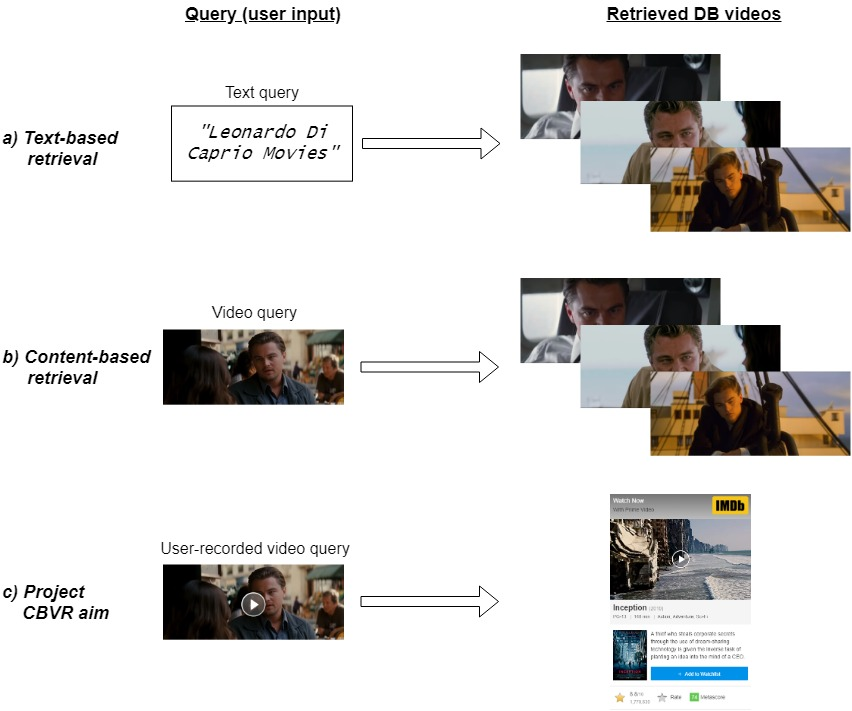
\includegraphics[width=\textwidth]{figures/content_text-retrieval_comparison.jpg}}
\caption{\label{fig:text_vs_content_retrieval}Illustrations of a text-based content-retrieval system \emph{(a)}, a content-based video retrieval system \emph{(b)}, and the project's desired CBVR system \emph{(c)}.}
\end{figure}

Content-based retrieval techniques quickly replaced text-based retrieval techniques towards the end of the 20th century by making use of the visual content to compute similarities between videos \cite{lai2015trajectory}. Instead of accepting a text string, the system takes a video as input to extract its visual contents, as shown in Figure \ref{fig:text_vs_content_retrieval}.\emph{b}. According to Petković et al. \cite{petkovic2000}, this visual content can be broken down into three different categories:
\begin{itemize}
    \item \textit{Raw data}, which corresponds to individual raw video frames and the video file's attributes such as the frame rate per seconds, the number of bits per pixel or the colour model used.
    \item \textit{Low-level visual content}  consists of the visual features that describe a video. This content includes colours, shapes, textures and motion. Low-level visual content can be extracted into histograms (see Section add-section) or features (see Section \ref{sec:features}) using a wide variety of existing techniques. Once the content has been extracted, it can be used to first compute similarities between videos \cite{lai2015trajectory} and later pattern match them.
    \item \textit{Semantic content} contains the high-level concepts that are present in a video. These high-level concepts can be described as objects or events using the features. To extract semantic content from a video, a grammar of rules for objects must be provided. An example of an object rule could be "if the shape is round, the colour is orange and the object is moving, then that object is a basketball".
\end{itemize}

In comparison to raw data, low-level visual content provides the most relevant visual information that can be extracted from a video for the purpose of a CBVR system. Semantic content extraction adds an additional layer of complexity compared to low-level visual content extraction as it requires domain knowledge and user interaction \cite{petkovic2000}. Therefore, this project will focus on using low-level visual content to extract information about the video and compute the similarities between the query video and database videos. It is important to note that this project's goal differs from classic CBVR systems where a list of videos is returned (see in Figure \ref{fig:text_vs_content_retrieval}.\emph{b}), as it must return a specific video that matches the most the query video (see Figure \ref{fig:text_vs_content_retrieval}.\emph{c}). To improve the pattern matching accuracy phase, raw data (e.g. audio) and metadata (e.g. captions) may be used to improve the pattern matching accuracy \cite{patel2012}.\\

% ----------------------------------------------------

\subsection{Temporal Aspects of Videos}
\label{sec:temporal-aspect-videos}

\subsubsection{Temporal Structure of a Video}

The most important difference between content-based image retrieval and video retrieval lies within the temporal aspect of the video. Naturally, the temporal aspect of a video clip stores supplementary information about the content, including dynamic low-level visual content e.g. an object's motion, and semantic content e.g. actions and events. According to A. Araujo et al. \cite{araujo2017i2v}, a video's temporal structure can be subdivided into three units, as shown in Figure \ref{fig:temporal_structure}:
\begin{itemize}
    \item \textit{Frames} correspond to the smallest temporal unit of a video file. A single segment of a video is referred to as a frame. Frames are also used to describe the frame rate (the frequency at which consecutive stills appear on a screen every second) e.g. ``24 fps'' corresponds to a video made up of 24 stills per second.
    \item \textit{Shots} are grouped sequences of visually similar frames. They are usually described  in seconds.
    \item \textit{Scenes} are a collection of shots which are related based on the action and objects present in the shot, thus giving them a semantic aspect. The length of a scene 
    is generally calculated in minutes rather than seconds.
\end{itemize}

\begin{figure}[h]
\centerline{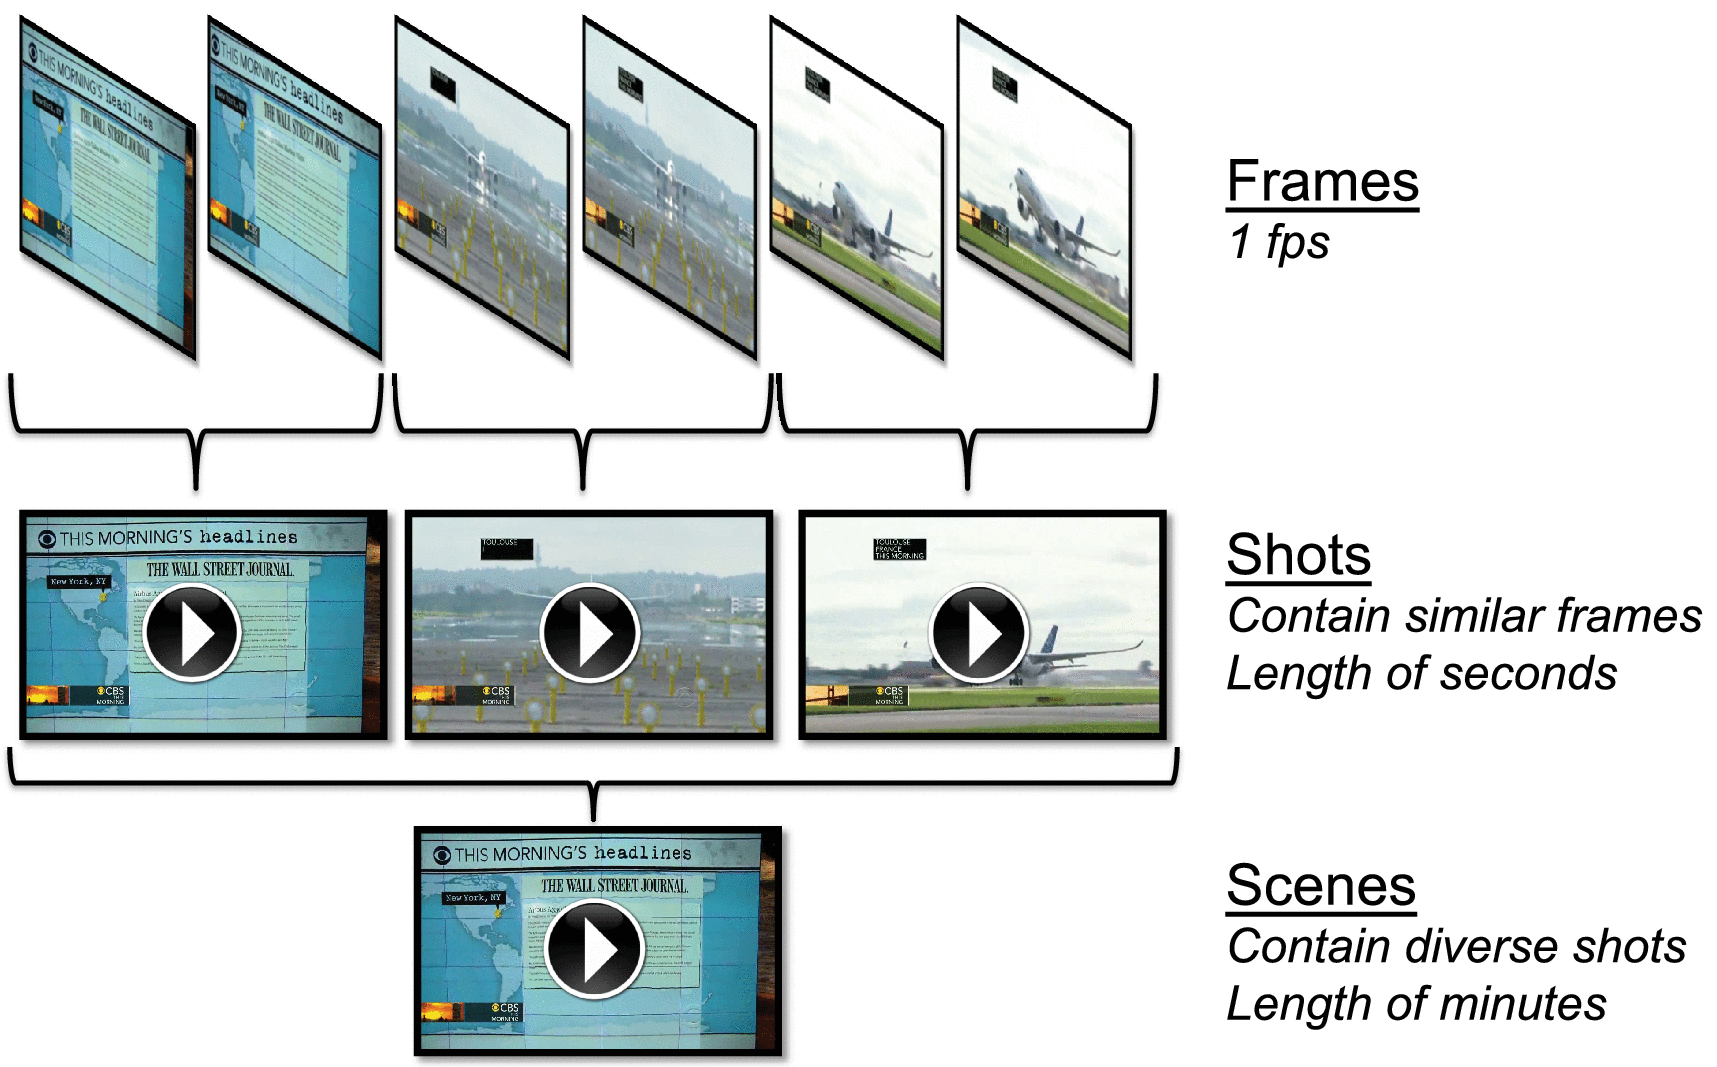
\includegraphics[width=0.75\textwidth]{figures/temporal_structure_videos.png}}
\caption{\label{fig:temporal_structure}Temporal structure of videos, including the different terms used to describe video temporal units. Figure courtesy of A. Araujo et al.}
\end{figure}

Because this project will explore possible solutions to create a CBVR system targeting databases of feature-length movies, a fourth video temporal structure category relevant to this project can be added to Araujo et al.'s initial list:
\begin{itemize}
    \item \textit{Movies} can be described as a large group of scenes that are used to tell a story. Movie durations commonly range from one to three hours.
\end{itemize}

\subsubsection{Challenges of Temporality}
\label{sec:cbvr-challenges}

Multiple challenges arise when dealing with CBVR systems in contrast to CBIR systems as the videos' temporal aspect adds a new dimension of complexity when extracting visual information. While the low-level visual content describing images remains mostly the same for videos (see Section ref-section), some new information that did not exist in images can be extracted, such motion. As mentioned previously, videos are a made up of frames, which make up shots when a combination of similar frames are played in succession. This means that videos carry information about motion, such as the trajectory of objects. This introduces unique challenges to the algorithms used to extract motion.\\

Because videos are made up of numerous stills, usually around 24 frames per second \cite{brownlow1980silentfilm}, two consecutive frames are near-identical. The pixels describing an object in one frame will remain the same in the next frame, except for the edge pixels perpendicular to the motion's trajectory \cite{bradski2008opencv}.\\

Figure \ref{fig:forrest_gump_frames} shows six frames from Forrest Gump's famous running shot, which lasts 44 seconds, making up a total of 1056 frames. Each frame in the figure was captured with 10-second intervals, meaning 240 frames separate each still. In the first three frames, the group of people running in the background barely moves in the space of 20 seconds. The pixels that describe the group in the shot remain mostly unchanged for all of the frames between the 3 samples, equivalent to 480 frames, with a few additional pixels describing the group as it advances towards the camera. The same can be said about the red cap in the last two frames. Most of the pixels making up the cap in the fifth frame remain the same in the sixth frame. This example perfectly betrays the reason why analysing a video frame by frame would be extremely inefficient when it comes to CBVR. Due to the similarities between consecutive frames, these should be aggregated \cite{araujo2017i2v} to describe a shot by using a selection of frames, such as taking the six frames in Figure \ref{fig:forrest_gump_frames} to describe the entire 44 seconds of video, rather than keeping the original 1056 frames to describe it.

\begin{figure}[h]
\centerline{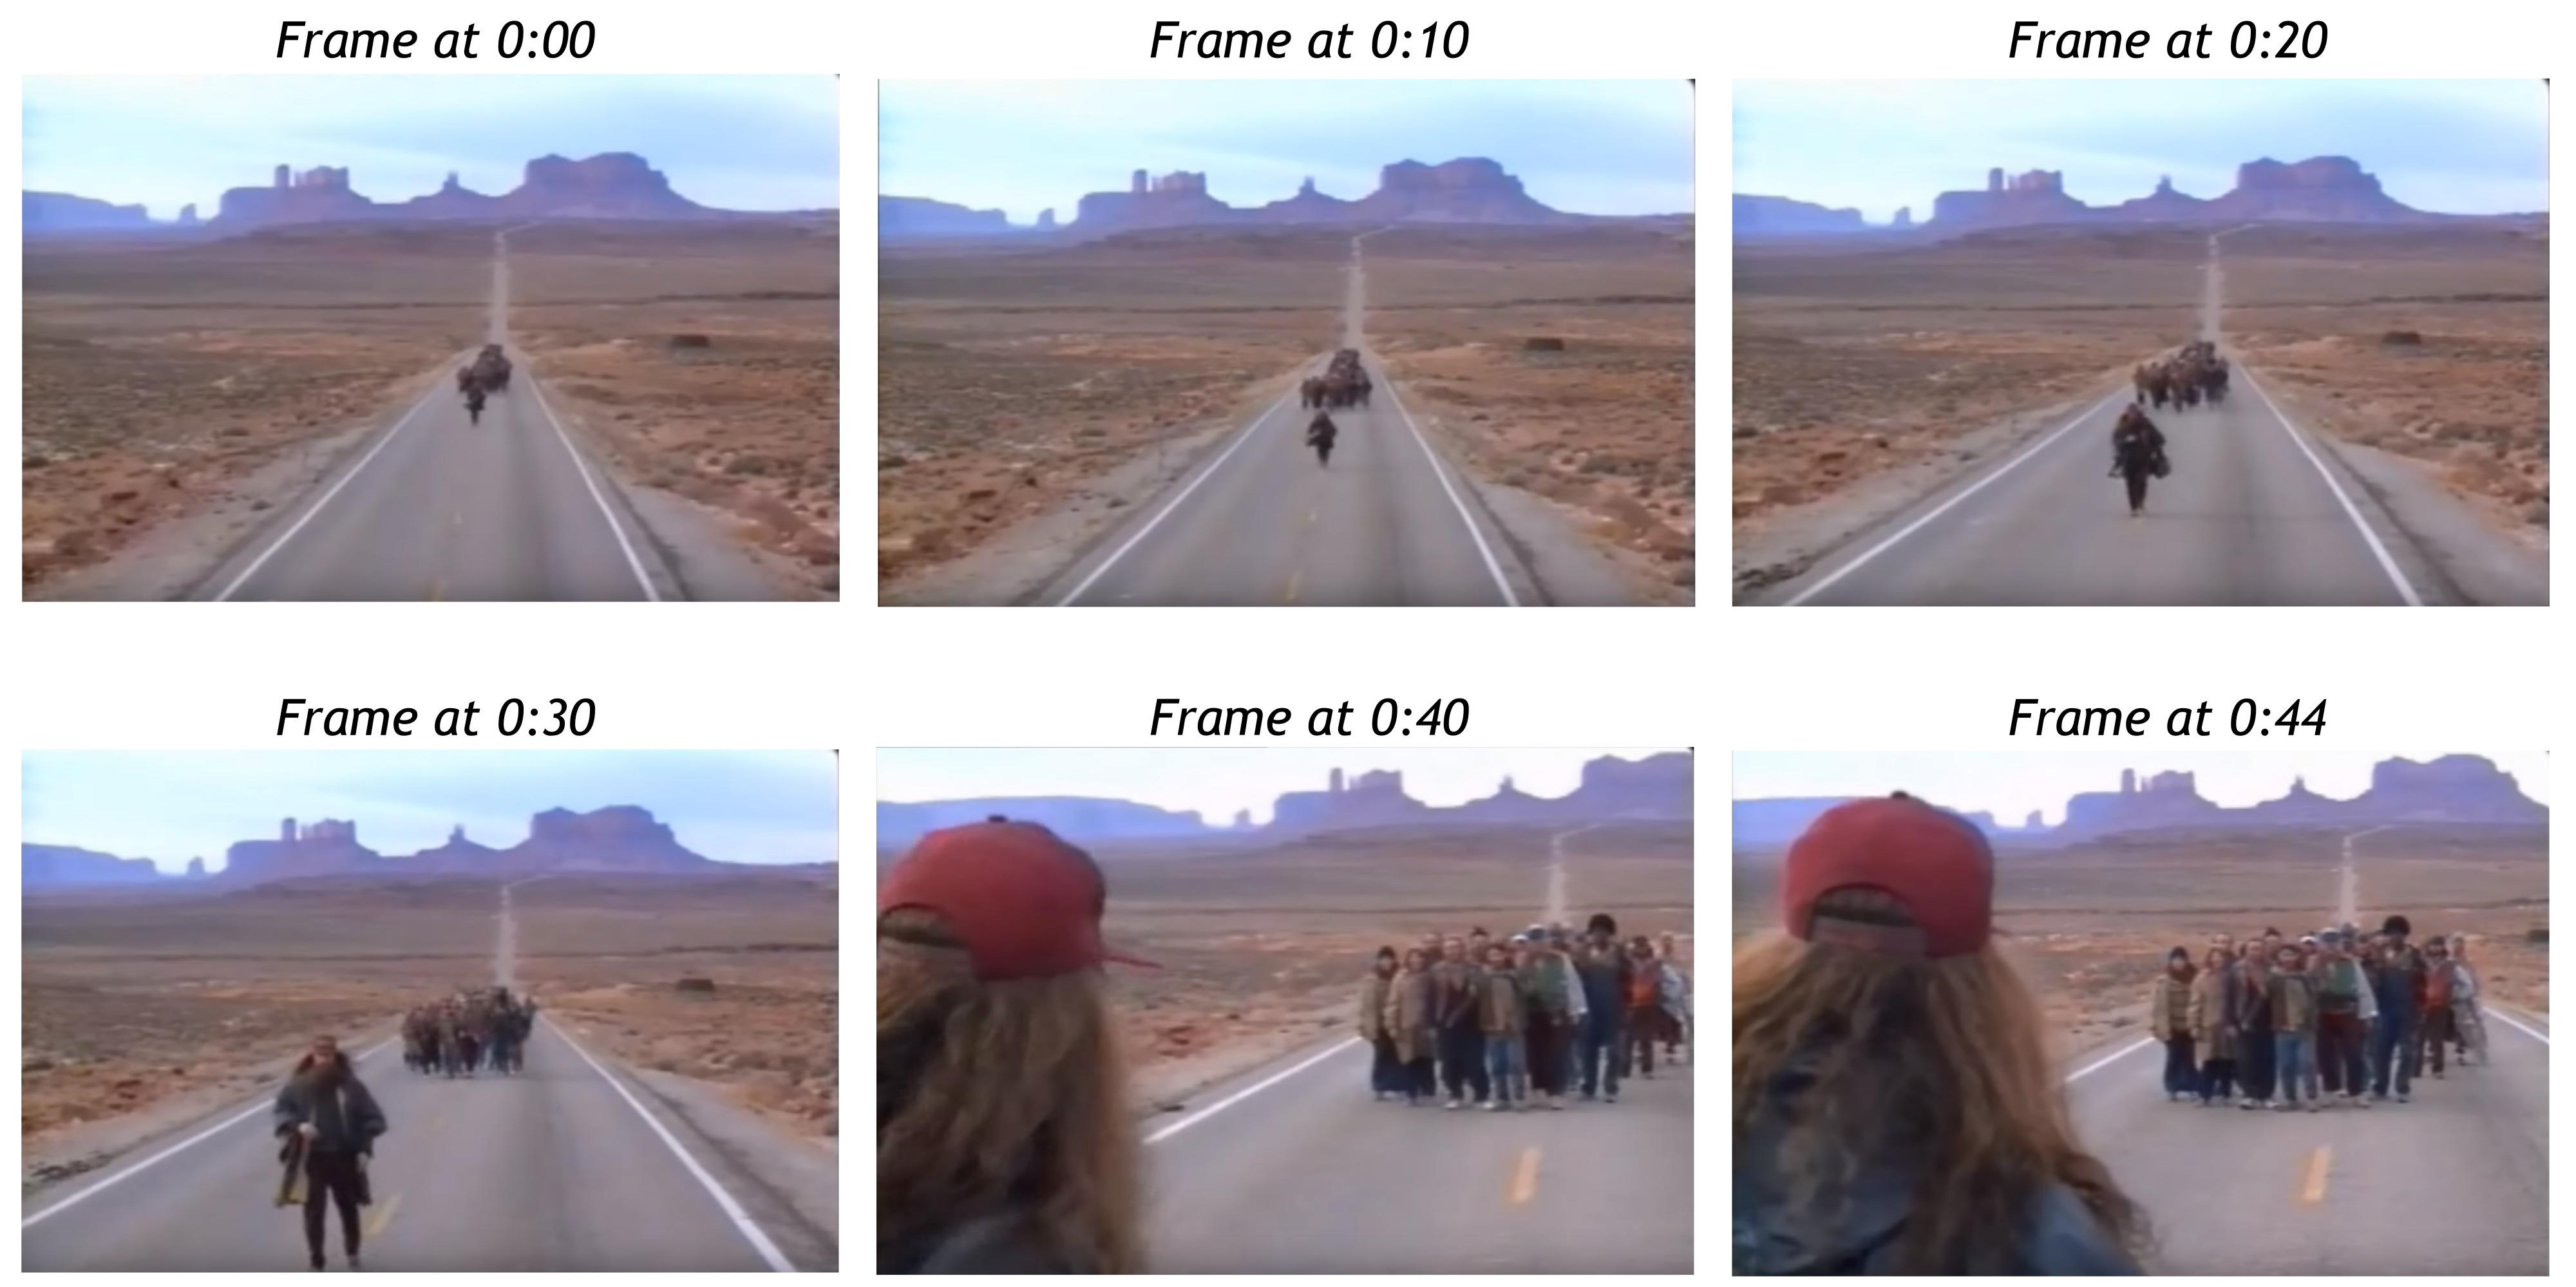
\includegraphics[width=\textwidth]{figures/forrest_gump_shot.jpg}}
\caption{\label{fig:forrest_gump_frames}Frames from the famous running scene in Forrest Gump extracted at intervals of 10 seconds. Video frames courtesy of \textit{``Forrest Gump long run scene"} YouTube video available online: \url{https://youtu.be/QgnJ8GpsBG8?t=325}.}
\end{figure}

\begin{comment}
    On top project aim mobile device using a database of feature-length movies.\\
    \cite{araujo2017i2v}One of the problems regarding video retrieval is the temporal aspect of the data. A solution to overcome the temporal aspect of the data is to aggregate each video into a compact signature to allow quicker and more efficient matching (when matching the query video to a video in the database).\\ 
    temporal aggregation problem of videos compared to images
\end{comment}

% ----------------------------------------------------

\subsection{CBVR for Mobile Devices}
\label{sec:mobile-cbvr-challenges}

The aforementioned project aim is for the system to work on mobile devices for two reasons. The first reason, as shown in Figure \ref{fig:wireframe} is to allow users to directly use their mobile phone to record the query video by pointing their camera to a screen displaying a movie, which will in turn tell them which movie is being played. Additional information retrieved from IMDb\footnote{Internet Movie Database}, such as cast, crew, ratings, runtime and synopsis could also be displayed. The second reason is the popularity of mobile devices, which may be due to the improvements made on mobile phones' processing power, allowing more tasks to be carried out through this medium. However, such a system on a mobile device causes many problems regarding the query video recording method and the computational power available on mobile devices.\\

\begin{figure}[h]
\centerline{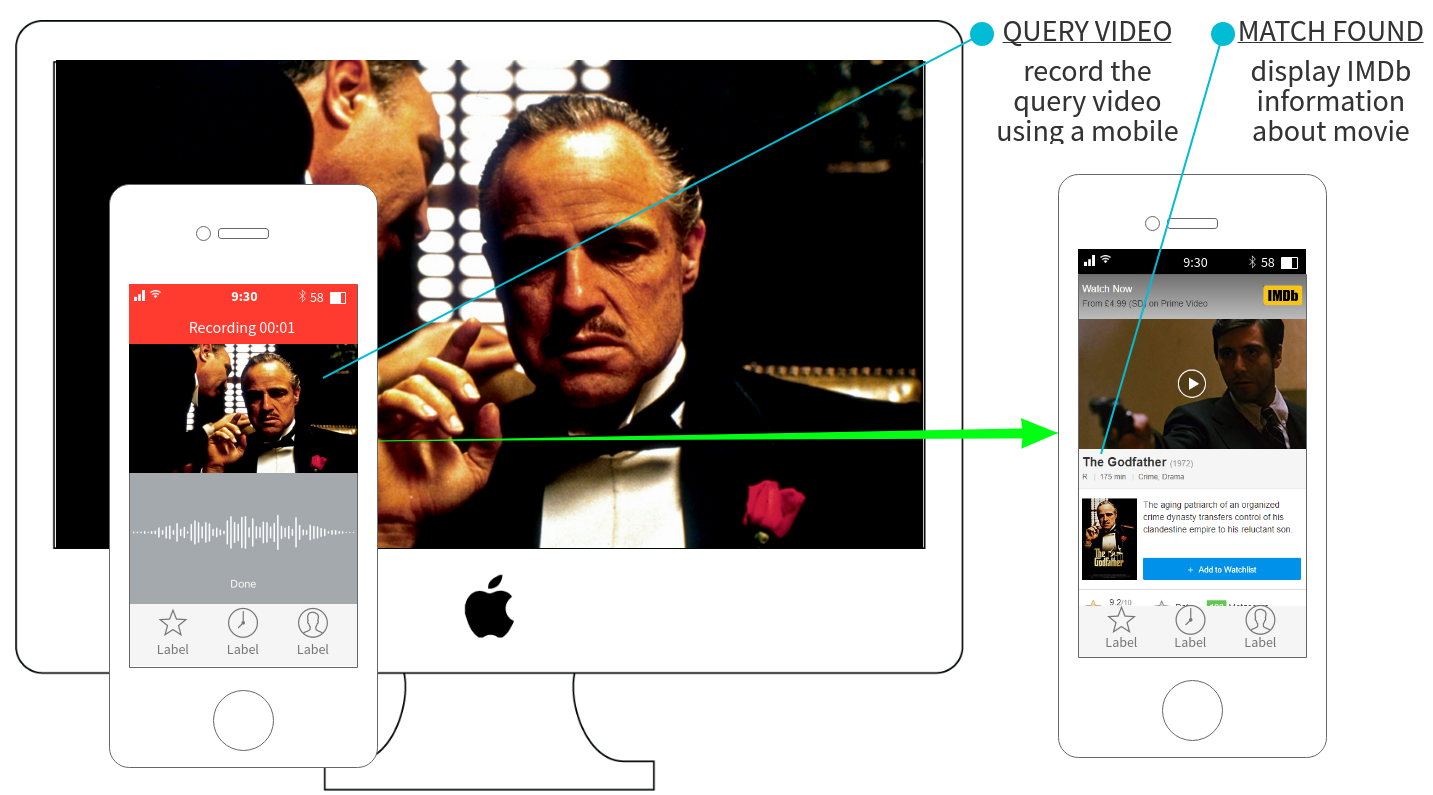
\includegraphics[width=1.25\textwidth]{figures/system_wireframe.png}}
\caption{\label{fig:wireframe}Wireframe showing the basic high-level concept of the system.}
\end{figure}

\subsubsection{Query Video Quality}
\label{sec:query-video-challenges}

Large visual differences are caused between the query clip and the actual clip stored in the database due to the capture conditions \cite{liu2014mobilevideosearch} \cite{wang2016actionregonition} such as:
\begin{itemize}
    \item Undesired camera movements due to unstable recording e.g. unstable recording, hand shaking.
    \item Low-quality recording due to poor user recording e.g. scaling and rotation, and due to the environment conditions e.g. lighting, reflections, blurring.
    \item Video noise because of the camera sensor.
    \item Decoding artefacts causes by various file compression.
\end{itemize}

These low-quality conditions add difficulty to the pattern matching phase where the similarities between the query video and database videos have to be computed. Indeed, if the query video is very different to the actual video, then the noisy elements of the video query must filtered out. For example, if the recorded video is shaky, then this shaking motion has to be pruned before analysing the recorded clip's motion. However, processing power must be used from the actual visual content extraction and pattern matching phases to be used for video noise filtering.

\subsubsection{User Experience}
\label{sec:user-experience}

According to Liu et al. \cite{liu2014mobilevideosearch}, the majority of mobile device users expect a polished product with quick video query and instant or progressive results, meaning that the searching algorithms must be efficient. However, one of the downsides of mobile devices is the computation power constraints. Despite the improvements of mobile processors, desktop devices still remain more powerful than mobile ones. A solution that Liu et al. suggest is to retrieve the low-level visual content locally on the mobile device, and send the query to a server where the pattern matching will take place \cite{liu2014mobilevideosearch}. This allows heavy computations to be off-loaded from the mobile device. Once a match is found, the result is returned to the user on his mobile device. A downside to this approach is the new constraint on network bandwidth rather than computational power.

\begin{comment}
    % todo - spread in sections above
    \subsubsection{Computational efficiency and database size}
    
    At the early stages of the development phase of the project, the database of videos for the system will be made up of shots only, lasting on average ten seconds. Longer videos will be used progressively based on the system's progress with shorter videos.\\
    mention \cite{hanjalic1999moviesegmentation}
    
    \cite{wang2016actionregonition}
    A challenge also lies within the computational power needed to process all the data in a database efficiently.\\
\end{comment}


%%%%%%%%%%%%%%%%%%%%%%%%%%%%%%%%%%%%%%%%%%%%%%%%%%%%%%%%%%%%%%%%%%%%%%%%%%%%%%%%%%
% 2 - VISUAL CONTENT EXTRACTION
%%%%%%%%%%%%%%%%%%%%%%%%%%%%%%%%%%%%%%%%%%%%%%%%%%%%%%%%%%%%%%%%%%%%%%%%%%%%%%%%%%
\section{Visual Content Extraction}

Extracting the visual content from a video allows this content to be used to describe videos and compute similarities between them. This visual content can be divided into two categories: static content and dynamic content. This section will first survey methods of extracting static content from videos, and will then focus on extracting dynamic content from videos.

% ----------------------------------------------------

\subsection{Static Content}
\label{sec:static-content}

Corresponds to content that can be extracted from a single frame from the video.
histograms
region-based content

% ----------------------------------------------------

\subsection{Dynamic Content}

Corresponds to content that requires the continuity between consecutive frames to be analysed.

\subsubsection{Features}
\label{sec:features}

Features correspond to specific visual objects or patterns in an image (or video frame). The low-level visual content aforementioned in Section \ref{sec:cbvr-methods} can be extracted into features, which store the visual descriptors of the video such as the colours and shapes \cite{petkovic2000} that make an object or a pattern unique. However, only good features features should be extracted from the image. It is therefore important to make the difference between good and poor features to only extract the useful ones. Figure \ref{fig:features_cube} shows an image of a 3D-shaped cube, along with coloured patches that make out potential features:
\begin{itemize}
	\item Blue features
	\item Green features
	\item Red features
\end{itemize}

\begin{figure}[h]
\centerline{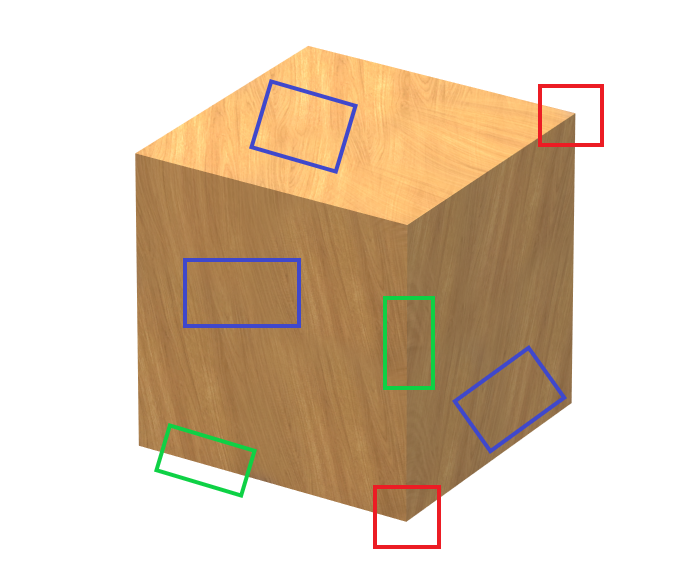
\includegraphics[width=0.5\textwidth]{figures/features_cube.png}}
\caption{\label{fig:features_cube}A 3D-shaped cube with coloured patches representing potential features.}
\end{figure}

Once good features like corners are extracted, they are used to compute visual similarities between the query video and the videos in the database. According to Petković et al., two types features can be extracted from a video: 
\begin{itemize}
    \item \textit{Static features} are used to characterise a frame from the video such as colours, shapes or textures. They can be used to describe images and videos.
    \item \textit{Dynamic features} describe a sequence of frames and therefore store the information regarding the temporal aspect of the video (See Section \ref{sec:temporal-aspect-videos}) such as objects' motions and trajectories.
\end{itemize}

Multiple techniques exist to retrieve a video's visual information to later compare it to the visual information stored in the database. This section will focus on Fisher Vectors, including the Bag-of-Words model that is necessary to understand Fisher Vectors.

\subsubsection{Finding features}
\label{sec:corner-detection}

TODO: Explain corner detection to find good features e.g. Harris Corner Detection

\subsubsection{Optical Flow}
\label{sec:optical-flow}

TODO:
\begin{itemize}
    \item Optical flow algorithms \cite{bradski2008opencv}:
    \begin{itemize}
        \item Dense Optical Flow
        \item Farneback Polynomial Expression Algorithms
        \item Lucas-Kanade Algorithm
    \end{itemize}
    \item Can calculate optical flow to prune camera movement caused by unstable recording e.g. hand shaking \cite{wang2016actionregonition}
\end{itemize} movements.

\begin{comment}
    Good matches when comparing low-level visual content can still produce poor results (60\% green and 40\% blue example) \cite{petkovic2000}
\end{comment}


%%%%%%%%%%%%%%%%%%%%%%%%%%%%%%%%%%%%%%%%%%%%%%%%%%%%%%%%%%%%%%%%%%%%%%%%%%%%%%%%%%
% 3 - PATTERN MATCHING METHODS
%%%%%%%%%%%%%%%%%%%%%%%%%%%%%%%%%%%%%%%%%%%%%%%%%%%%%%%%%%%%%%%%%%%%%%%%%%%%%%%%%%
\section{Pattern Matching Methods}

Retrace evolution of pattern matching methods: BoW to CNN (and before? --> find surveys)

% ----------------------------------------------------

\subsection{Bag-of-Words Model}

TODO:
\begin{itemize}
    \item Explain how Bag-of-Words model works
    \item H. Wang's implementation of BoW histogram \cite{wang2016actionregonition}
    \item State that Fisher Vectors are an improvement on BoW
\end{itemize}

% ----------------------------------------------------

\subsection{CNN}

CNNs


%%%%%%%%%%%%%%%%%%%%%%%%%%%%%%%%%%%%%%%%%%%%%%%%%%%%%%%%%%%%%%%%%%%%%%%%%%%%%%%%%%
% 4 - DATABASE VIDEO PRE-PROCESSING
%%%%%%%%%%%%%%%%%%%%%%%%%%%%%%%%%%%%%%%%%%%%%%%%%%%%%%%%%%%%%%%%%%%%%%%%%%%%%%%%%%
\section{Database Video Pre-Processing}

The database of videos can be pre-processed to later optimise the pattern matching phase, enabling the overall system to operate more efficiently.

% ----------------------------------------------------

\subsection{Key Frames}
\label{sec:key-frames}

Y. S. Heo et al. \cite{heo2016colortransfer} suggests only considering key frames in videos to operate on. These key frames would be used for the feature extraction, database pre-processing and pattern matching phases. Key frames are determined based on the difference between two consecutive frames using the histogram chi-square distribution approach (See Equation \ref{eq:chisquare}).\\

\cite{heo2016colortransfer}
This approach only considers key frames from the query video clip. Key frames are determined based on the difference between two consecutive frames using the histogram chi-square distribution approach (See Equation \ref{eq:chisquare}).\\

TODO:
\begin{itemize}
    \item Explain histogram chi square distribution technique.
    \item When the amount of differences $\theta$ between two frames exceeds a threshold, usually set at the empirical value $\theta = 0.005$, then the current frame is set as a key frame.
\end{itemize}

\begingroup \Large \begin{equation} \label{eq:chisquare}
    C(h^{t-1}, h^{t}) = \sum_{i=0}^{255} \frac{(h_{i}^{t-1} - h_{i}^{t})^2}{h_{i}^{t-1} + h_{i}^{t}}
\end{equation} \endgroup \\

To illustrate the advantage of using key frames, let's use a 3-seconds long shot recorded at 30 fps\footnote{Frames Per Second} of a ball rolling on the ground, which would consist of a total of 90 frames. Analysing all the frames individually as stills would be highly inefficient. However, selecting key frames to work on, as depicted in Figure \ref{fig:rolling_ball} where a single frame is chosen for each second, would means that 3 key frames can be used for feature extraction and pattern matching instead of using all of the 90 frames that make up the video.\\

\begin{figure}[h]
\centerline{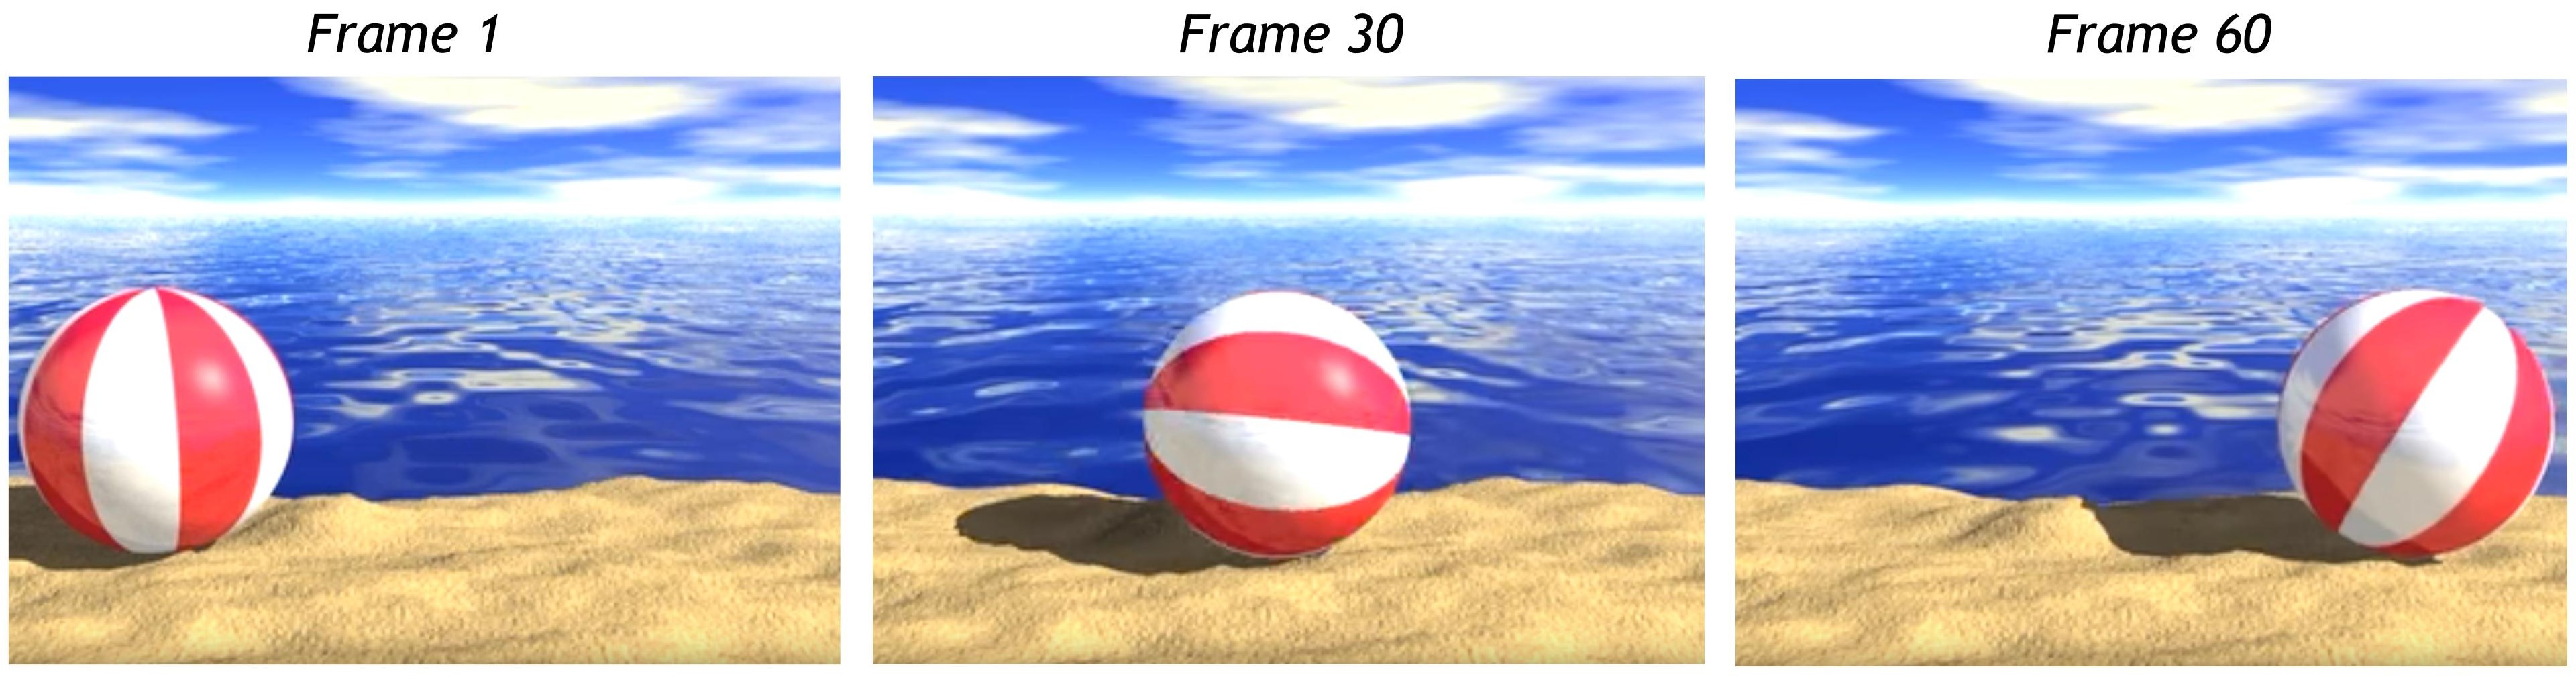
\includegraphics[width=\textwidth]{figures/ball_rolling.jpg}}
\caption{\label{fig:rolling_ball}Example of frames to sample for low-visual content analysis. The first frame for each second (one frame every thirty seconds) is retrieved for a 30 fps 3-second video of a ball rolling from the left-hand side of the screen to the right-hand side. Video frames courtesy of \textit{``How to Animate a Rolling Ball"} YouTube video available online: \url{https://youtu.be/cgbLAreElNI?t=130}.}
\end{figure}

% ----------------------------------------------------

\subsection{Thumbnails}
\label{sec:thumbnails}

In their work, M. Okabe et al. \cite{okabe2018animating} generate thumbnails for each video in their database, which are stored as additional data along with the origin video file. The thumbnails for the query video and for the database videos would be generated using the same algorithm in order to create similar results. This technique can be used in parallel to A. Araujo et al.'s \cite{araujo2017i2v}, who states that an initial shortlist of potentially matching videos can be generated before the main pattern matching phase. This shortlist can be created by computing the similarities between the query video's thumbnail and the database video's thumbnails. Many advantages can be gained from this small initial step which could be extremely important in the overall system's speed and efficiency:
\begin{itemize}
    \item Videos that share no similarities to the query video will not be considered at all during the main pattern matching phase e.g. if the query video corresponds to a colourful sunset, then database videos of cloudy environments will be immediately filtered out as it is unlikely that they will match with the query video in the main pattern matching phase.
    \item This initial step is extremely speedy as it only uses a single still that describes the entire video. Therefore the entire process will not be noticeably slowed down, although this only applies for relatively small databases.
    \item The database videos' thumbnails will have already been generated during the database's pre-processing phase, which only occurs a single time.
\end{itemize}

This solution works well for shots, but work less well for scenes and movies (See Figure \ref{fig:temporal_structure}). Indeed, shots can be characterised by a single image as they are only made up of similar frames. However, the visual content describing the shots that make up scenes (and movies) can be very different from each other. A possible solution could be to create a thumbnail for each shot in a scene, and store each thumbnail in a list. For example, if a scene contains six different shots, then six thumbnails will be generated to describe that scene.\\

\begin{comment}
\cite{okabe2018animating}
For quicker pattern matching and feature extraction, 16 pixels separate two feature points, allowing for rough pattern matching rather than exact pattern matching. This could be used when using feature-length movies as database videos to pattern match.
\end{comment}

% ----------------------------------------------------

\subsection{Movie Segmentation}
\label{sec:movie-segmentation}

TODO:
\begin{itemize}
    \item A. Hanjalic et al. \cite{hanjalic1999moviesegmentation}
\end{itemize}

% ----------------------------------------------------

\subsection{Trajectory Analysis}
\label{sec:trajectory-analysis}

TODO:
\begin{itemize}
    \item Similar trajectories: if the dynamic features of a video are used to find similarities, then the database of videos can be pre-analysed to detect trajectories \cite{lai2015trajectory}
    \item Use of optical flow in this particular case
\end{itemize}

% ----------------------------------------------------

\subsection{Fisher Vectors}
\label{sec:fisher-vectors}

TODO:
\begin{itemize}
    \item Fisher Vectors can be used to generate a compact signature for videos, which will then be used for computing similarities between the query video's FV and the database videos' FVs \cite{araujo2017i2v}
\end{itemize}